
\documentclass[10pt,a4paper]{report}
%\usepackage[latin1]{inputenc}
\usepackage[utf8]{inputenc}
\usepackage{amsmath}
\usepackage{amsfonts}
\usepackage{amssymb}
\usepackage{graphicx}
\usepackage{multicol}
\usepackage{tabularx}
\usepackage{tikz}
\usetikzlibrary{arrows,shapes,automata,petri,positioning,calc}
\usepackage{hyperref}
\usepackage{tikz}
\usetikzlibrary{matrix,calc}
\usepackage[margin=0.5in]{geometry}
% ---- power functions -----% 
\newcommand{\myvec}[1]{\ensuremath{\begin{pmatrix}#1\end{pmatrix}}}
\let\vec\mathbf

\providecommand{\norm}[1]{\left\lVert#1\right\rVert}
\providecommand{\abs}[1]{\left\vert#1\right\vert}
\let\vec\mathbf

\newcommand{\mydet}[1]{\ensuremath{\begin{vmatrix}#1\end{vmatrix}}}
\providecommand{\brak}[1]{\ensuremath{\left(#1\right)}}
\providecommand{\lbrak}[1]{\ensuremath{\left(#1\right.}}
\providecommand{\rbrak}[1]{\ensuremath{\left.#1\right)}}
\providecommand{\sbrak}[1]{\ensuremath{{}\left[#1\right]}}
%-------end power functions----%
\newenvironment{Figure}
  {\par\medskip\noindent\minipage{\linewidth}}
  {\endminipage\par\medskip}
\begin{document}
%--------------------logo figure-------------------------%
\begin{figure*}[!tbp]
  \centering
  \begin{minipage}[b]{0.4\textwidth}
 
\includegraphics[scale=0.05]{../../Downloads/iitlogo.jpg} 
  \end{minipage}
  \hfill
  \vspace{5mm}\begin{minipage}[b]{0.4\textwidth}
\raggedleft  
\includegraphics[scale=0.10]{../../Downloads/nrc.jpeg} 

  \end{minipage}\vspace{0.2cm}
\end{figure*}
%--------------------name & rollno-----------------------
\raggedright \textbf{Name}:\hspace{1mm} YADATI KRISHNA\hspace{3cm} \Large \textbf{Assignment-4}\hspace{2.5cm} % 
\normalsize \textbf{Roll No.} :\hspace{1mm} FWC22036\vspace{1cm}
\begin{multicols}{2}

%----------------problem statement--------------%
\raggedright \textbf{Problem Statement:}\vspace{2mm}
\raggedright \\Slope of a line passing through P(2,3) and intersecting the line x+y=7 at a distance of 4 units from P  .\\
\vspace{5mm}

%-----------------------------solution---------------------------
\raggedright \textbf{SOLUTION}:\vspace{2mm}\\

%---------given----------------%
\raggedright \textbf{Given}:\vspace{2mm}\\
Equation of line is x+y=7 \\\vspace{1mm}
\begin{align}
P=(2,3)
\end{align}


%-------------To find ------------------%
\textbf{To Find }\vspace{2mm}\\
Slope of the line passing through P(2,3) \vspace{5mm}  \\ 
%--------------steps----------------------%
\textbf{STEP-1}\vspace{2mm}\\

Let $\vec{A}$ be any point on the line and the coordinates are,\vspace{1mm}
\begin{align}
    \vec{A}=\myvec{
    4\\
    3
    } 
\end{align}
 \vspace{2mm}
From given, we know that point $\vec{P}$ \\
\begin{align}
    \vec{P}=\myvec{
    2\\
    3
    } 
\end{align} \vspace{2mm}
Let $\vec{m}$ be the directional vector \\\vspace{1mm}
\begin{align}
    \vec{m}=\myvec{
    1\\
    -1
    } 
\end{align}
Given distance from point $\vec{P}$ to the line is 4\\
\vspace{5mm}
\textbf{STEP-2}\vspace{2mm}\\
The distance from a point  $\vec{P}$ to the line is given by, \\ \vspace{1mm}
\begin{align}
	\label{dist_3d_def}
	d\brak{\lambda } &=\norm{\vec{A} + \lambda \vec{m}-\vec{P}}
\end{align}
 \vspace{1mm}

Squaring on both the sides \\ \vspace{2mm}
\begin{align}
 	d^2\brak{\lambda } &=\norm{\vec{A} + \lambda \vec{m}-\vec{P}}^2
\end{align}
\vspace{2mm}

\textbf{STEP-3}\vspace{2mm}\\
After substituting $\vec{A}$ , $\vec{P}$ and $\vec{m}$ in the above equation and solving (6) we get 
\begin{align}
{\lambda }=1.64, -3.64
\end{align}

Using equation (7) any point on the line  
 \begin{align}
	\label{eq:dir_line}
	\vec{x} = \vec{A} + \lambda \vec{m}
\end{align}
substituting $\vec{A}$ and $\vec{m}$ in (8) we get\\
\vspace{1mm}
\begin{align}
	\label{eq:dir_line}
	\vec{x1} = \myvec{
	0.36\\
	6.64
	}
\end{align}\\
and
\begin{align}
	\label{eq:dir_line}
	\vec{x2} = \myvec{
	5.64\\
	1.36
	}
\end{align}\\
using (9) and (10) in line equation we get\\
\begin{center}
2.21x+y=8.66\\
x+2.21y=7.42
\end{center}

\begin{center}
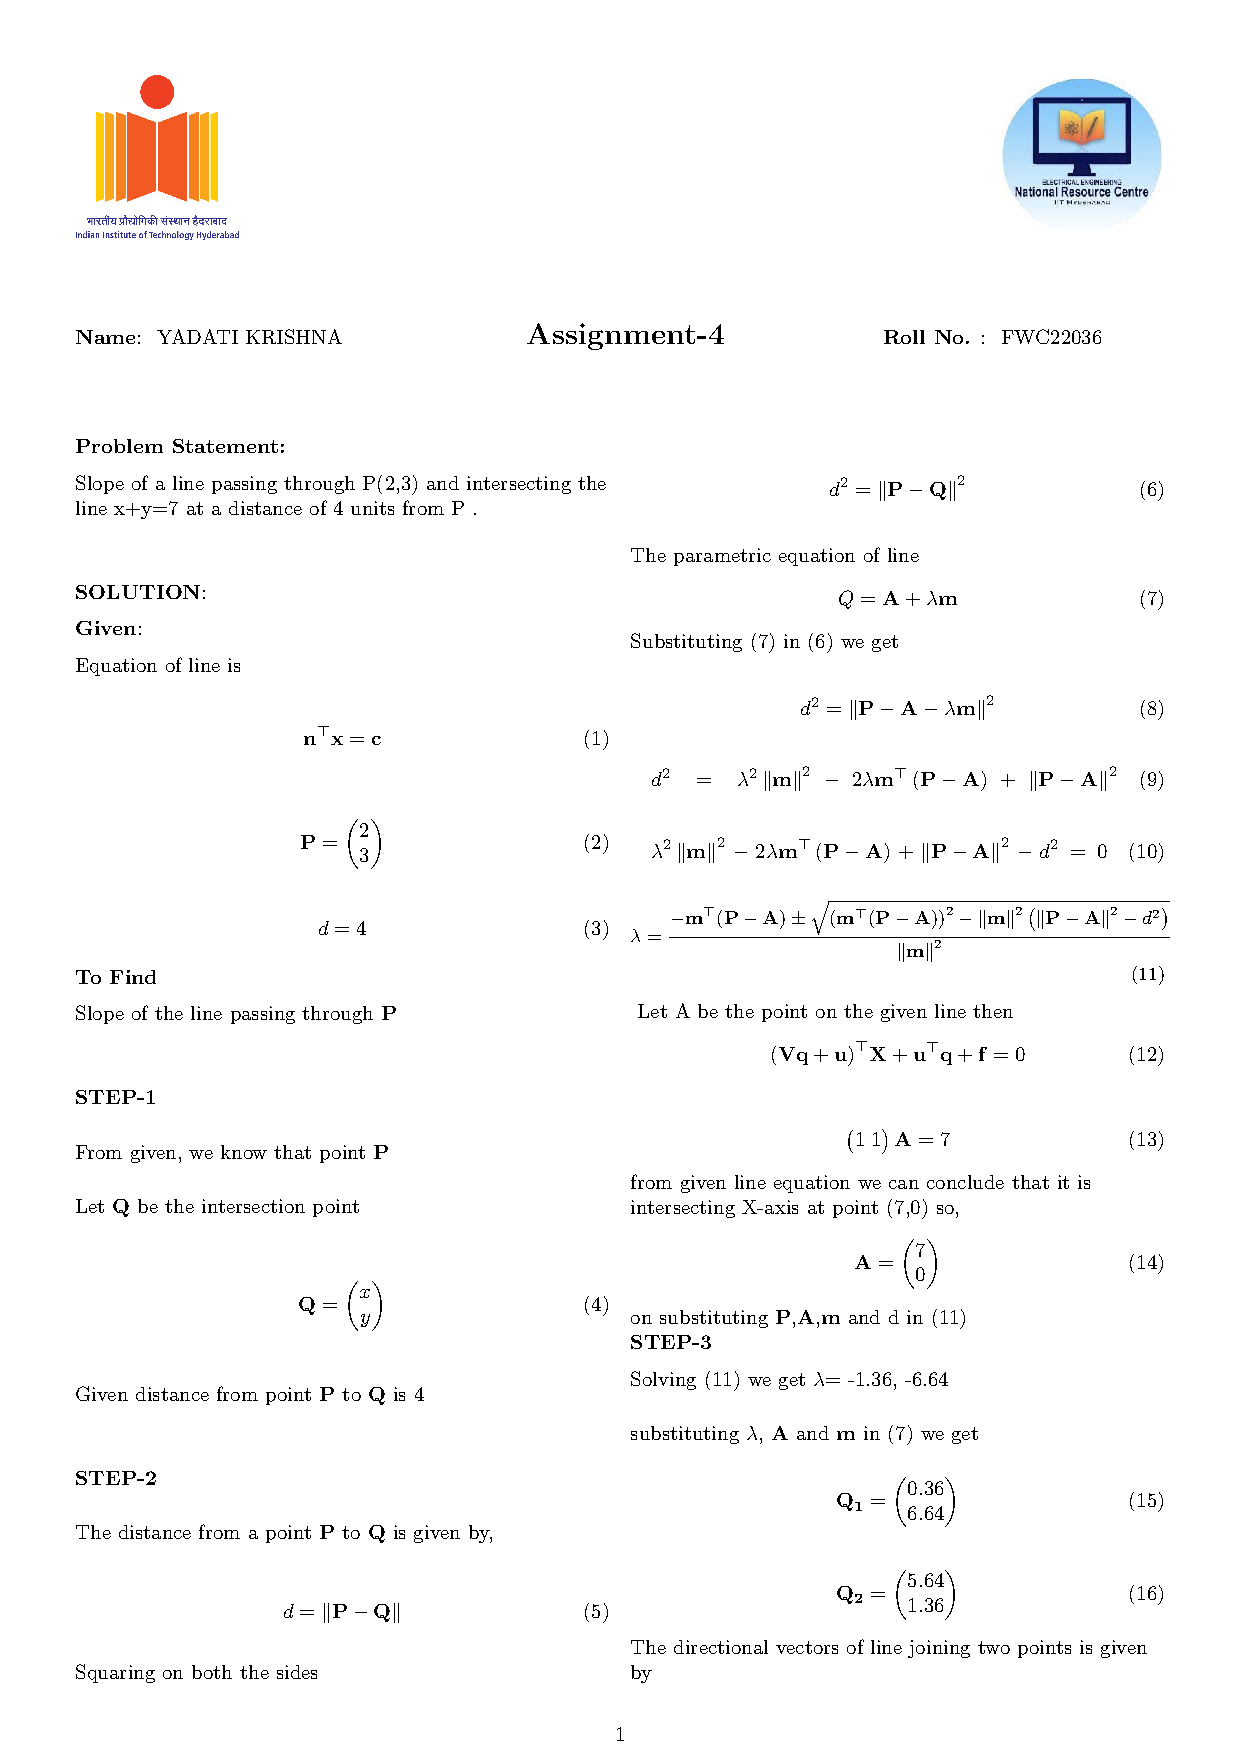
\includegraphics[scale=0.6]{../python/figs/line1.pdf}  
 \end{center}\vspace{1mm}
 
 \vspace{2mm} \textbf{Construction}
\begin{center}
\setlength{\arrayrulewidth}{0.5mm}
\setlength{\tabcolsep}{6pt}
\renewcommand{\arraystretch}{1.5}
    \begin{tabular}{|l|c|}
    \hline 
    \textbf{vertex} & \textbf{coordinates} \\ \hline
   $\vec{P}$ & $\myvec{
   2\\
   3
   } $ \\\hline
  
      \end{tabular}
  \end{center}
  
\raggedright  Download the code \\
Github link: \href{https://github.com/KrishnaYadati/Assignments/blob/main/Matrix-line_assignment/line_program/line1.py}{Assignment-4}.
  \end{multicols}
\end{document}
